\scanpage{3}
\uline{Structure à l'$\infty$ des $M_{g,\nu}$}

\begin{tabular}{r p{0.79\linewidth} r}
1. & Courbes standard & 1 \\
2. & Graphe associé à une courbe standard\newline \unsure{Maquettes} & 3 \\
3. & Courbes stables, et MD-graphes & 6 \\
4. & Le théorème de Mumford-Deligne & 10 \\
5. & Spécialisation de MD-graphes & 15 \\
6. & Morphismes de générisation de graphes et de \unsure{maquettes} & $16'$ \\
7. & Étude des $\widehat M_{g,\unsure{\nu}}$ de dim $\leq 2$ : a) détermination des graphes correspondants & 25 \\
8. & Structure \unsure{de|des} spécialisation des strates en dim. modulaire ambiante $\leq \unsure{4}$ & $29'$ \\
9. & Structure groupoïdale \deleted{des} multiplicités modulaires de Teichmüller compactes (la MDT-structure) : Construction, morphismes de générisation & 37 \\
10. & Structure MDT analytique : \unsure{action} des morphismes de normalisation entre MD-graphes & 45 \\
11. & Digression : déploiement d'un diviseur à croisements normaux. Structure à l'infini des groupoïdes fondamentaux & 52 \\
12. & Digression (suite) : types canoniques associés à une stratification par croisements normaux, et leur dévissage en ``types élémentaires'' & 74 \\
13. & Digression sur stratifications \inserted{``locales''} générales & 86
\end{tabular}
\mspage{2}
\scanpage{4}
Structure à l'infini des $M_{g,\nu}$

1. \uline{Courbes \unsure{standard|standart}}.

Soit $k$ un corps alg. clos. Une ``courbe \unsure{standard|standart}'' sur $k$ est un\deleted{e \unsure{courbe}} schéma $X$ sur $k$ satisfaisant les conditions suivantes :

a) $X$ quasi-projectif, \inserted{toute composante irréd. est} de dim $1$

b) Tout point de $X$ est soit lisse, soit un ``point quadratique'' (``ordinaire'') -- i.e. isom. (loc. ét) à la courbe $\operatorname{Spec}(k[X,Y]/XY)$ au point $0$.

Il est connu qu'on peut donner une unique ``complétion'' $\widehat X$ de $X$, telle que \inserted{$\widehat X$ soit un schéma propre, \unsure{que}} $X$ s'identifie à un ouvert dense de $\widehat X$, et que $\widehat X$ soit lisse en les pts de $\widehat X\setminus X=I$. Alors $\widehat X$ est une courbe projective, $I$ est \deleted{\unsure{contenu}} une partie finie de $\widehat X(k)$ contenue dans l'ens. ouvert des pts de lissité de $\widehat X$. L'ens. $A$ des pts singuliers de $X$ s'identifie à l'ens. analogue pour $\widehat X$
\[
(1)\qquad
\left\{\begin{aligned}
I&=\widehat X\setminus X\subset\widehat X^{\mathrm{lisse}}(k)
&&\text{``pts à l'infini'' de }X\\
A&=X\setminus X^{\mathrm{lisse}}=\widehat X\setminus\widehat X^{\mathrm{lisse}}\subset X(k)
&&\text{(pts singuliers de }X\text{)}
\end{aligned}\right.
\]
La donnée de $X$ équivaut à celle de
\mspage{3}
\scanpage{5}
$(\widehat X,I)$, où $\widehat X$ est un schéma projectif, dont \unsure{tte} composante irréductible est de dim $1$, et dont l'ensemble singulier est formé de pts quadratiques ordinaires -- et $I$ est un sous-schéma fini étale de $\widehat X^{\mathrm{lisse}}$, ou ce qui revient au $=$, une partie finie de $\widehat X^{\mathrm{lisse}}(k)$.

Soit $\widetilde{\widehat X}=\widehat{\widetilde X}$ le normalisé de $\widehat X$, \deleted{alors}
\[
\widetilde I=\widehat{\widetilde X}\setminus\widetilde X
=\text{Image inverse de }I\text{ par }\widetilde{\widehat X}\to\widehat X
\]
l'ens. des \deleted{ses} ``points à l'infini'' de $\widetilde X$, on a
\[
(2)\qquad\widetilde I\xrightarrow{\sim}I
\]
et nous identifions généralement $\widetilde I$ et $I$, et plus généralement \deleted{$\unsure{\widehat X^{\mathrm{lisse}}}$ \unsure{à}} les pts de $\widehat X^{\mathrm{lisse}}$ aux pts correspondants de $\widetilde{\widehat X}$. Soit $\widetilde A$ l'image inverse de $A$ dans $\widetilde X$ (ou dans $\widehat{\widetilde X}$), alors
\[
(3)\qquad\widetilde A\longrightarrow A
\]
est une application de degré $2$, d'où une involution sans pts \unsure{fixe|fixes} $\sigma_{\widetilde A}$ dans $\widetilde A$.

Ainsi, à la courbe \unsure{standard|standart} $X$ nous avons associé \unsure{le système|les systèmes} de données
\mspage{4}
\scanpage{6}
\mspage{2}
suivant :
\[
(4)\quad\left\{\begin{aligned}
&\text{a) Une courbe projective et lisse }Y(=\widehat{\widetilde X})\deleted{\unsure{sur }k}\\
&\text{b) Deux parties }\inserted{\text{finies}}\text{ disjointes }\widetilde A\text{ et }I\text{ de }Y(k)\\
&\text{(ou encore, deux sous-schémas finis étales}\\
&\text{disjoints }\widetilde A_k\text{ et }I_k\text{ de }Y\text{)}\\
&\text{c) Une involution sans point fixe }\sigma_{\widetilde A}\text{ de}\\
&\widetilde A\text{ (qui est donc de cardinal pair).}
\end{aligned}\right.
\]
Inversement, partant de données a) b) c), on construit une courbe \unsure{standard|standart} $X$ en passant au quotient dans $Y\setminus I_k\supset\widetilde A_k$ par l'involution $\sigma$ -- i.e. $X$ est universel \inserted{(dans (Sch))} pour la donnée $p$ :
\diagram{\begin{tikzcd}
Y\setminus I_k\arrow[r,"p"] & X\\
\bigl(\,\widetilde A_k\arrow[u,"i"]\arrow[ur,dashed] & \bigr)
\end{tikzcd}}
, soumise à $(pi)\sigma=pi$.

Ainsi la catégorie des courbes \unsure{standard|standart} sur $k$ \inserted{(pour les iso)} apparaît comme équivalente à celle des systèmes a) b) c) ci-dessus. (pour les iso)\ldots

\uline{NB} On récupère $\widehat X$ comme quotient de $Y$ par $\sigma$.
\mspage{5}
\scanpage{7}
\uline{Généralisation sur une base quelconque.}

Une \uline{courbe \unsure{standard|standart}} sur $S$ (multiplicité schématique, disons) sera \unsure{définie|défini} constructivement en termes d'un système a) b) c) \inserted{comme} ci-dessus, i.e.
\[
(5)\quad\left\{\begin{aligned}
&\text{a) }Y,\text{ schéma propre et lisse }\inserted{\text{sur }S}\text{ partout de}\\
&\text{dim relative }1;\\
&\text{b) }\widetilde A\text{ et }I,\text{ deux sous-schém. de }Y,\\
&\text{finis étales sur }S,\quad\deleted{\unsure{\text{avec}}}\ \widetilde A\cap I=\varnothing;\\
&\text{c) }\sigma_{\widetilde A}\text{ une involution de }\widetilde A,\text{ opérant}\\
&\text{librement.}
\end{aligned}\right.
\]
On construit alors $\widehat X=\unsure{Y}/\sigma$, contenant $A\simeq\widetilde A/\sigma$ et $I$ comme sous-schémas \inserted{fermés} finis étales sur $S$, et on définit $X=\widehat X\setminus I$. On peut montrer que le foncteur
\[
(6)\qquad(Y,\widetilde A,\inserted{I,}\sigma_{\widetilde A})\longmapsto X
\]
\margin{\uline{NB} NB ce foncteur est compatible aux images inverses\ldots}
des systèmes (5) (pour les iso) vers les schémas relatifs, \inserted{(pour les iso)} est \uline{pleinement fidèle}.
\margin{faux tel quel !}
\mspage{6}
\scanpage{8}
\mspage{3}
\margin{Le foncteur est pl. fid. au mieux sur une base $S$ réduite -- faux p. ex. sur les \unsure{nbs} duaux d'un corps (si $I\neq\varnothing$). Pour avoir un foncteur pl fidèle, il faut \unsure{se placer} dans le contexte \uline{propre}, i.e. \unsure{remplacer} $X$ par $(\widehat X,I)$ (de sorte que $X=\widehat X-I$).}
J'appelle ``courbe \inserted{relative} \unsure{standard|standart}'' sur $S$, tout élément de l'image essentielle. Le système $(Y,\widetilde A,I,\sigma)$ qui lui donne naissance s'appellera le ``complété normalisé'' \inserted{(relatif)} (par abus de \deleted{système définissant} langage, puisque c'est non seulement le schéma relatif $Y$, mais $Y$ avec la structure supplémentaire $\widetilde A,I,\sigma_{\widetilde A}\ldots$).

2. \uline{Graphe associé à une courbe \unsure{standard|standart}.}

Revenons au cas d'un corps de base $k$ alg. clos, pour commencer. Soit $\unsure{X}$ une courbe \unsure{standard|standart}, d'où $Y,\deleted{\unsure{\widetilde A},}I,\widetilde A,\sigma_{\widetilde A}$.

Posons
\[
(7)\qquad S=\pi_0(Y)\simeq\text{ens. des comp. irréd. de }X
\]
On a alors le diagramme d'applications canoniques entre ensembles finis
\[
(8)\qquad
\diagram{\begin{tikzcd}
& I\arrow[d,"p"]\\
\widetilde A\arrow[r,"\unsure{o|\sigma}"]\arrow[d,"q"'] & S\\
A=\widetilde A/\sigma &
\end{tikzcd}}
\]
\mspage{7}
\scanpage{9}
où $q$ est de degré $2$ et définit l'involution $\sigma_{\widetilde A}$. Les applications $o$ et $p$ sont induites par les inclusions $\widetilde A\hookrightarrow Y$, $I\hookrightarrow Y$ en passant aux $\pi_0$.

Le système
\diagram{\begin{tikzcd}
\bigl(\widetilde A\arrow[r,"o"] & S,\sigma_{\widetilde A}\bigr)
\end{tikzcd}}
ou
\diagram{\begin{tikzcd}
\bigl(\widetilde A\arrow[r,"o"]\arrow[d,"\text{deg 2}"'] & S\bigr)\\
A &
\end{tikzcd}}
, peut être considéré comme définissant un \uline{graphe}, dont $S$ est l'ens. des sommets, et $\widetilde A$ l'ens. des \uline{arcs} (ou arêtes orientées) l'application $o$ étant l'application ``origine d'un arc''. Ce graphe ne dépend que de $\widehat X$, pas de $X$ i.e. du choix de $I\subset\widehat X(k)$. C'est pour tenir compte de ce choix que l'on considère, en plus de la structure de graphe, la donnée supplémentaire
\[
(9)\qquad I\longrightarrow S
\]
\mspage{8}
\scanpage{10}
\mspage{4}
Le graphe indique comment les composantes irréductibles de $X$ (\unsure{figurées|figurés} par les sommets) se rencontrent deux à deux -- les pts d'intersection, i.e. les pts singuliers (\inserted{``doubles'', \unsure{sc.}}quadratiques) de $X$, correspondent aux arêtes. Si une composante irréductible $X_\alpha$ de $X$ correspond au sommet $\alpha$ du graphe, alors les boucles fermées en $\alpha$ correspondent biunivoquement aux pts doubles de $X_\alpha$ -- donc dire que les $X_\alpha$ sont lisses signifie que le graphe $G_X$ n'a pas de boucles fermées, i.e. que pour tt arc, l'origine est $\neq$ de l'extrémité.

Il est clair que tout graphe fini peut être obtenu \inserted{(à iso près)} \deleted{à l'aide} par une $\widehat X$ convenable -- et $\unsure{=|\overline m}$ avec des \unsure{compo-}
\mspage{9}
\scanpage{11}
santes $X_\alpha$ de genre \inserted{$g_\alpha$} donné (i.e. des $\widetilde X_\alpha$ de genre $g_\alpha\ldots$). De plus, quand on se donne \deleted{\unsure{des}} $I\to S$ ($I$ ens fini), cela peut être réalisé par un $I\subset\widehat X^{\mathrm{lisse}}$, i.e. par une courbe \unsure{standard|standart} $S$.

La \uline{maquette} d'une courbe \unsure{standard|standart} $X$ consiste, par définition, en les données suivantes
\[
(10)\quad\left\{\begin{aligned}
&\text{a) le graphe }G_X=\biggl(
\underset{\inserted{\substack{\Vert\\\pi_0(\widetilde X)\\\Vert\\\pi_0(\widehat{\widetilde X})}}}{S},
\underset{\inserted{\substack{\Vert\\\unsure{\operatorname{Sing}(X)}}}}{\widetilde A},
\underset{\deleted{\unsure{\widehat X}}}{\sigma_{\widetilde A}}
\biggr)\\
&\text{b) L'}\deleted{\text{application}}\inserted{\text{ensemble}}\ I=\widehat X\setminus X,\text{ et l'application}\\
&\qquad I\longrightarrow S\\
&\text{c) L'application}\\
&\qquad S\xrightarrow{\uline{g}}\mathbb N\\
&\qquad\alpha\longmapsto\text{genre de }Y_\alpha=\widehat{\widetilde X}_\alpha
\end{aligned}\right.
\]
Une structure formée d'un graphe fini $G$\inserted{$=(S,\widetilde A,\sigma_{\widetilde A})$}, d'un ensemble fini $I$ \deleted{\unsure{de}} au dessus de l'ens. des sommets $S$ de $G$, et d'une application \inserted{``genre''} : $S\xrightarrow{\uline{g}}\mathbb N$, sera
\mspage{10}
\scanpage{12}
\mspage{5}
appelé ici une ``maquette''.

\uline{Proposition} \inserted{Considérons la maquette d'une courbe \unsure{standard|standart} $X$.}
a) Soient $\alpha,\beta\in S$, alors $\alpha,\beta$ appartiennent à la $=$ composante conn. du graphe $G$, ssi. $X_\alpha$ et $X_\beta$ appartiennent à la $=$ comp. conn. de $X$. Donc \deleted{\unsure{l'on}} on a une bij. can.
\[
(11)\qquad\pi_0(G_X)\simeq\pi_0(X),
\]
en particulier $X$ est connexe ssi $G_X$ est connexe.

b) Supposons $X$ connexe i.e. $\widehat X$ connexe, i.e. $H^0(\widehat X,\underline O_{\widehat X})\unsure{\xleftarrow{\sim}|\simeq}k$ i.e dim $H^0(\widehat X,\underline O_{\widehat X})=1$.

Posons \deleted{$g(X)=\dim H^1(X,\underline O_X),\quad\chi(X)=\chi$}
\[
(12)\quad\left\{\begin{aligned}
g(\widehat X)&=\dim H^1(\widehat X,\underline O_{\widehat X})\\
\chi_{\mathrm{coh}}(\widehat X)&=\chi(X\deleted{\unsure{g}},\underline O_X)=1-g(X)
\end{aligned}\right.,
\]
on a alors
\[
(13)\quad\chi_{\mathrm{coh}}(\widehat X)
=\deleted{\unsure{\sum_{\alpha\in S}\chi_{\mathrm{coh}}(\widehat{\widetilde X}_\alpha)}}
\inserted{\chi(\widetilde{\widehat X})-\underbrace{\operatorname{card}A}_{\mu}}
=\sum_{\alpha\in S}(1-g_\alpha)-\mu
\]
i.e.
\[
(14)\quad\left\{\begin{aligned}
g(\widehat X)&=\sum g_\alpha+(-\operatorname{card}S+\underbrace{\operatorname{card}A}_{\mu}+1)\\
&=\sum g_\alpha+h_1
\end{aligned}\right.,
\]
\mspage{11}
\scanpage{13}
où \deleted{$\unsure{h_1}$ \unsure{est le}}
\[
(15)\qquad h_1=\operatorname{rg}_{\mathbb Z}H_1(G_X,\mathbb Z).
\]
\uline{Démonstration} \unsure{Standard|Standart} (!) -- la formule (13) résulte d'une suite exacte \inserted{\unsure{standard|standart}} de cohomologie reliant $\underline O_{\widehat X}$, $\underline O_{\widetilde{\widehat X}}$ et les singularités de $\widehat X$, d'ailleurs la formule d'EP pour le graphe $G_X$ nous donne
\[
\chi(G_X)=\underbrace{h_0}_{1}\deleted{\unsure{(G_X)}}-h_1=\operatorname{card}S-\operatorname{card}A
\]
i.e.
\[
1-\operatorname{card}S+\operatorname{card}A=h_1\qquad\text{O.K.}
\]
\uline{Corollaire} Le nb $g(\widehat X)$ ne dépend que de la maquette de $X$, par la formule (14)
\[
g(\widehat X)=\underbrace{\sum_{\alpha\in S}g(\alpha)+h_1}_{\overset{\mathrm{dfn}}{=}\ \text{genre de }G}
\]
-- on l'appelle le \uline{genre} de la maquette.

On appelle \uline{type} de la maquette le couple $(\unsure{\bar g|g},\nu)$, où $g$ est son genre et $\nu=\operatorname{card}I$ est le \uline{poids marqué}. On appelle \uline{poids marqué} d'un sommet l'entier naturel
\mspage{12}
\scanpage{14}
\mspage{6}
\margin{c'est le nb de pts à l'infini de la composante $X_\alpha$}
$\operatorname{card}I_\alpha$ (où $I_\alpha$ est la fibre de $I$ en $\alpha\in S$)
\[
(16)\qquad\nu_\alpha=\operatorname{card}I_\alpha,
\]
et on appelle \uline{poids total} d'un sommet l'entier
\[
(17)\qquad\widehat\nu_\alpha=\nu_\alpha+
\underset{\substack{\Vert\ \mathrm{déf}\\
\text{ordre du sommet }\alpha,\\
\text{i.e. }\operatorname{card}\widetilde A_\alpha,\text{ où }\widetilde A_\alpha\text{ est la fibre}\\
\text{de }\widetilde A\text{ au dessus de }\alpha,\text{ i.e. le}\\
\text{nb d'arcs sortant de }\alpha}}{\omega_\alpha}
\]
c'est donc le nb de ``pts marqués'' (provenant de pts doubles \unsure{et} de pts à l'infini de $X$) sur la composante $Y_\alpha$ de $Y=\widetilde{\widehat X}$.

3. \uline{Courbes ``stables''.} \uline{et} \uline{MD-graphes.}

Une courbe \unsure{standard|standart} \inserted{(sur $k$ alg. clos)} est ``stable'', si elle satisfait à l'une des conditions équivalentes suivantes

a) $\operatorname{Aut}X$ est fini

b) Pour tout $\alpha$, $(Y_\alpha,I_\alpha\cup\widetilde A_\alpha)$ est anabélien
\[
\text{i.e.}\quad 2g_\alpha+\widehat\nu_\alpha\geq3\qquad
\text{i.e.}\quad 2g_\alpha-2+\widehat\nu_\alpha\geq1,\quad\text{i.e.}
\]
\mspage{13}
\scanpage{15}
1°) Si $g_\alpha=1$, on a $\widehat\nu_\alpha\geq1$

2°) Si $g_\alpha=0$ on a $\widehat\nu_\alpha\geq3$

c) Tout champ de vecteurs sur $Y$ nul sur $\deleted{\unsure{\widetilde A}}I\cup\widetilde A$ est nul.

d) $\underline{\operatorname{Aut}}_{(Y,\widetilde A_k,I)}$ est un schéma en groupes fini étale sur $k$.

On voit que cette condition (sous la forme b)) ne dépend que de la \uline{maquette} de la courbe. On dit que $X$ est une \uline{MD-courbe} (MD, initiales de ``Mumford-Deligne'' -- ou de ``modulaire'') si elle est stable, et \inserted{0-}connexe \inserted{(i.e. connexe non vide)}.

Les maquettes de telles courbes sont les maquettes $0$-connexes \inserted{et} stables (i.e. dont les sommets de genre $1$ sont de poids total $\geq1$, et les sommets de genre $0$ sont de poids total $\geq3$), on les appellera les MD-graphes.

\uline{NB} Une maquette est un MD-graphe ssi

a) elle est $0$-connexe (i.e. le graphe $G$ est conn. $\neq\varnothing$)

b) elle n'est pas réduite à un seul sommet de genre $1$, de poids total $0$ (pas d'arête, pas de points marqués)

c) les sommets de genre $0$ sont de poids total $\geq3$.
\mspage{14}
\scanpage{16}
\mspage{7}
\uline{Proposition} Si $(G=(S,\widetilde A,\sigma),I,g:S\to\mathbb N)$ est un MD-graphe, son type $(g,\nu)$ est anabélien, i.e. $2g+\nu\geq3$.

Si on avait $g=1$, $\nu=0$, alors la relation
\[
g=1=\sum g_\alpha+h_1
\]
montre que ou bien tous les $g_\alpha$ sont nuls, et $h_1=1\deleted{\unsure{+1}}$, ou bien tous les $g_\alpha$ sauf un \inserted{$g_{\alpha_0}$} sont nuls, et $g_{\alpha_0}=1$, $h_1=0$ \inserted{(i.e. $G$ est un arbre)}. \inserted{Dans le premier cas,} La relation $s_0-s_1=h_0-h_1=1-1=0$ montre qu'il y a autant de sommets que d'arêtes, dans le deuxième, $s_0-s_1=1-0=1$ il y a un sommet de plus que d'arêtes.

Mais la relation $\nu=0$ implique que les sommets de genre $0$ sont d'ordre $\geq3$. \inserted{$G$ n'est pas réduit à un sommet, puisqu'il est stable de type $(1,0)$.} Mais un \deleted{graphe top. compact \unsure{ou}} \inserted{arbre qui \unsure{n'est réduit} à un seul sommet} a au moins deux bouts, dont l'un au moins sera de genre $0$, ce qui élimine le cas 2°. Donc tous les sommets sont de genre nuls \inserted{(donc aucun sommet n'est un bout)} et $h_1=\unsure{1}$. Mais \deleted{\unsure{comme}} un graphe topologique $0$-connexe avec $h_1=1$ qui n'a pas de \inserted{pt.} bord topologique est homéomorphe au cercle, donc s'il est réalisé par un graphe combinatoire, tous les sommets de celui-ci sont d'ordre $2$, ce qui contredit qu'ils soient d'ordre trois.
\mspage{15}
\scanpage{17}
Éliminons de $=$ le cas $g=0$, $\nu\leq2$. Ici $g=0=\sum g_\alpha+h_1$ implique que les $g_\alpha$ et $h_1$ sont nuls : tous les sommets sont de genre $0$, le graphe est un arbre. Il ne peut être réduit à un seul sommet, donc il a au moins deux bouts, dont les \unsure{poids} marqués doivent être $\geq2$, donc \deleted{\unsure{le}} on a $\nu\geq2+2=4$, absurde.

Soit $G$ une \deleted{\inserted{MD-}graphe}\inserted{maquette}. On dit qu'une \deleted{\inserted{MD-}} courbe \deleted{\unsure{standard|standart}}\inserted{\unsure{standard|standart}} $C$ sur un corps alg. clos est de \uline{type $G$}, si sa maquette est iso à $G$, on dit qu'elle est \inserted{$G$-}\uline{épinglée} si on se donne un iso entre sa maquette et $G$ (c'est donc une structure suppl. sur $\unsure{C|X}$, appelée $G$-épinglage).

Soit $(\widehat X,I)$ une courbe \unsure{standard|standart} sur une base $S$ quelconque, on dit qu'elle est de type $G$ si ses fibres géom. sont de type $G$. Alors les \deleted{\unsure{``types'' des}}\inserted{maquettes} des
\mspage{16}
\scanpage{18}
\mspage{8}
fibres géom. de $(\widehat X,\underline I)$ forment les fibres d'un schéma en maquettes \inserted{(ou en MD-graphes)} sur $\unsure{\mathcal S|S}$
\[
(\deleted{\unsure{\underline G|\underline S}}\underline S,\underline{\widetilde A},\sigma_{\underline{\widetilde A}},\underline I,\ \underline{\widetilde A}\to\underline S,\ \underline I\to\underline S,\ \inserted{\underline S\xrightarrow{\underline g}\mathbb N_{\mathcal S}})
\]
(système de rev. finis étales \inserted{de $\mathcal S$} et de morphismes entre ceux-ci), loc. isomorphes à la maquette $G$ donnée. \deleted{\unsure{Le}} On appelle \inserted{$G$-}épinglage de $(\widehat X,\underline I)$ tout isomorphisme entre $G_{\mathcal S}$ et $\underline G(\widehat X,\underline I)$. Si \deleted{$\unsure{\Gamma}$}
\[
(18)\qquad\Gamma=\operatorname{Aut}G
\]
(groupe fini), les $G$-épinglages de $(\widehat X,\underline I)$ s'identifient aux sections d'un certain $\Gamma_{\mathcal S}$-torseur, \deleted{\unsure{qui est le|qui sera le}}\inserted{appelé} \uline{torseur des $G$-épinglages} de $(\widehat X,\underline I)$.

Considérons, sur une base $\mathcal S$ fixée, la catégorie \inserted{(pour les iso)} des courbes standard $G$-épinglées. Pour tt $\alpha\in S$ (ens. des sommets de la maquette) soit $\widehat I_\alpha=I_\alpha\amalg\widetilde A_\alpha$ l'ensemble (de cardinal $\widehat\nu_\alpha=\text{poids total de }\alpha$) somme
\mspage{17}
\scanpage{19}
des fibres $I_\alpha$ et $\widetilde A_\alpha$ de $I$ et $A$ au dessus de $\alpha$. La donnée d'une courbe \unsure{standard|standart} $G$ épinglée sur $\mathcal S$ équivaut à la donnée, \deleted{de} pour $\forall\ \alpha\in S$, d'une courbe relative (propre lisse \inserted{relt} $0$-connexe) $Y_\alpha$ sur $\mathcal S$, de genre relatif $g_\alpha$, \uline{et} d'un \inserted{$\mathcal S$-}mono. $(\widehat I_\alpha)_{\mathcal S}\hookrightarrow Y_\alpha$.

Désignons, \deleted{par $\mathcal M_{g_\alpha,\deleted{\nu_\alpha}\inserted{\widehat I_{\unsure{\alpha}}}}$} pour \deleted{\unsure{de}}\inserted{un} entier naturel $g\deleted{\unsure{\alpha}}$ et un ens. fini $I$ (de cardinal $\nu$) par
\figure{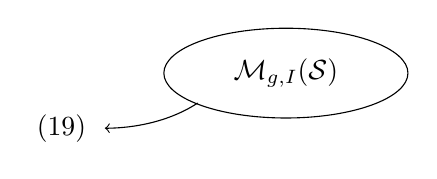
\begin{tikzpicture}[baseline=(m.base)]
\node (m) at (0,0) {$\mathcal M_{g,I}(\mathcal S)$};
\draw (0,0) ellipse (1.55 and .57);
\draw[->] (-1.12,-.38) .. controls (-1.55,-.66) and (-2.05,-.7) .. (-2.3,-.7);
\node at (-2.85,-.7) {$(19)$};
\end{tikzpicture}}
le \deleted{catégorie}\inserted{groupoïde} des courbes relatives $Y$ (propres, lisses, $0$-connexes) sur $\mathcal S$, \uline{$I$-ponctuées} i.e. munies d'un mono. $I_{\mathcal S}\hookrightarrow Y$. On trouve donc, si
\[
(20)\qquad\mathcal M_G(\mathcal S)
\]
désigne le groupoïde des courbes \unsure{standard|standart} $G$-épinglées sur $\mathcal S$, une équivalence
\[
(21)\qquad\mathcal M_G(\mathcal S)\simeq\prod_{\alpha\in S}\mathcal M_{g_\alpha,\widehat I_\alpha}(\mathcal S).
\]
\mspage{18}
\scanpage{20}
\mspage{9}
Cette équivalence est compatible avec les chgts de base, et avec le transport de structure pour $G$ variable.

On voit alors que pour que, pour $\mathcal S$ variable, le champ en groupoïdes
\[
(22)\qquad\mathcal S\longrightarrow\mathcal M_G(\mathcal S)
\]
soit $2$-représentable par une étendue schématique, il f. et s. qu'il en soit de $\unsure{=|\overline m}$ des
\[
\mathcal S\longrightarrow\mathcal M_{g_\alpha,\widehat I_\alpha}(\mathcal S),
\]
ce qui signifie aussi que les types correspondants $(g_\alpha,\widehat\nu_\alpha)$ sont anabéliens, i.e. que la maquette $G$ est stable. Si on suppose \inserted{déjà} $G$ $0$-connexe, cela signifie donc précisément que $G$ est un MD-graphe. On désignera alors par $\mathcal M_G$ la multiplicité modulaire
\mspage{19}
\scanpage{21}
correspondante, \deleted{que} de sorte qu'on aura un iso can.
\margin{plutôt, une \uline{équivalence}}
\[
(23)\qquad\mathcal M_{\unsure{G}}\simeq\prod_\alpha\mathcal M_{g_\alpha,\widehat I_\alpha}.
\]
Notons que $\Gamma=\operatorname{Aut}G$ opère sur $\mathcal M_G$ de façon évidente, et aussi sur le système $(\widehat I_\alpha,g_\alpha)_{\alpha\in S}$ donc sur le deuxième mb de (23), qui est un iso. compatible aux op. de $\Gamma$.

On peut considérer la multiplicité mixte
\[
(24)\qquad(\mathcal M_G,\Gamma)=\mathcal M_{[G]},
\]
qui a priori ne dépend que du type d'isomorphie $[G]$ de $G$, et qui s'interprète, en termes de ce dernier, comme la multiplicité schématique modulaire pour le groupoïde fibré (sur la $2$-cat. des multiplicités schématiques) des courbes \unsure{standard|standart} relatives de type $[G]$.
\mspage{20}
\scanpage{22}
\mspage{10}
\margin{$(g,\nu=\operatorname{card}J)$ anabélien}
\uline{NB} Si $\operatorname{card}J=\nu$, alors $\mathcal M_{g,J}$ est isomorphe au schéma modulaire $\mathcal M^!_{g,\nu}$ (via un iso. $[1,\nu]\cap\mathbb Z\simeq J$), de façon compatible avec les autom. des groupes $\unsure{\mathfrak S_J|\mathfrak G_J}$ et $\unsure{\mathfrak S_\nu|\mathfrak G_\nu}$. On sait que $\mathcal M^!_{g,\nu}$ est lisse de type fini sur $\mathbb Z$. Il en est donc de $\unsure{=|\overline m}$ de $\mathcal M_{g,J}$, donc aussi de $\mathcal M_G$ (pour $G$ semi-stable) et de $\mathcal M_{[G]}=(\mathcal M_G,\Gamma)$.

4. \uline{La théorie de Mumford-Deligne}

Soient $\mathcal S$ une multiplicité schématique, $\unsure{\mathcal X|\mathfrak X}$ un \deleted{courbe} schéma relatif sur $\mathcal S$, propre sur $\mathcal S$, $\underline I$ un sous-schéma fermé de $\mathcal X$. On dit que $(\mathcal X,\underline I)$ est une MD-courbe relative sur $\mathcal S$, si $\mathcal X,\underline I$ sont plats de présentation finie sur $\mathcal S$, et si pour $\forall$ pt géom. de $\mathcal S$, la
\mspage{21}
\scanpage{23}
fibre $(\mathcal X_{\bar s},\underline I_{\bar s})$ est une \inserted{MD-}courbe géométrique sur $\unsure{k(s)|\kappa(s)}$ -- i.e. $\mathcal X_{\bar s}$ est $0$-connexe, de dim $1$, \deleted{\unsure{ainsi q.}} les pts singuliers sont \inserted{$\notin I_{\bar s}$ et sont} des pts doubles ordinaires, et enfin la condition de rigidité infinitésimale \inserted{(en automorphismes)} est satisfaite -- \deleted{donc} i.e. on exige que $\mathcal X_{\bar s}$ ne soit pas de genre $1$ lisse avec $I_{\bar s}=\varnothing$, \unsure{et} que les comp. irréd. de genre $0$ de $\mathcal X_{\bar s}$ soient de ``poids marqué''
\[
\geq 3.
\]
La différence avec les considérations du n° précédent, c'est que maintenant ($\unsure{=|\overline m}$ sur une base $\mathcal S$ connexe, p.ex. \deleted{$\unsure{\mathcal S=}$} un trait) les \uline{types} des fibres géométriques peuvent varier d'un pt géom. à un autre. Mais il est clair que le type \uline{numérique} $(g,\nu)$ ne change pas (invariance de $\chi(\widehat X_s,\underline O_{\widehat X_s})\ldots$ et de $\operatorname{card}\underline I_s$), plus précisément,
\margin{\illegible{1}\ \deleted{\illegible{1}}}
\mspage{22}
\scanpage{24}
\mspage{11}
c'est une fonction localement constante sur $\mathcal S$.

Fixons nous un type numérique $(g,\nu)$\inserted{\uline{anabélien} $(2g+\nu\geq3)$}, et considérons, pour $\mathcal S$ variable, le groupoïde fibré
\[
(24)\qquad\mathcal S\longmapsto\widehat{\mathcal M}_{g,\nu}(\mathcal S)=\begin{gathered}\text{MD-courbes}\\\text{relatives sur }\mathcal S,\text{ de}\\\text{type numérique}\\\text{égal à }(g,\nu)\end{gathered}
\]
On a alors le vraiment \unsure{mirifique} théorème suivant :

\margin{On suppose $2g+\nu\geq3$ (cas anabélien)}
\uline{Théorème de Mumford-Deligne} : Le

\figure{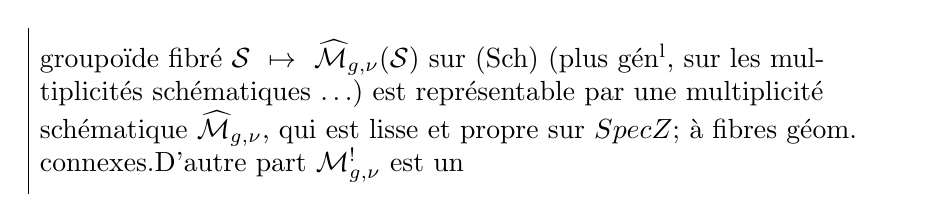
\begin{tikzpicture}
\node[anchor=north west,text width=0.9\linewidth,align=left,inner sep=4pt] (T) at (0,0) {
groupoïde fibré $\mathcal S\mapsto\widehat{\mathcal M}_{g,\nu}(\mathcal S)$ sur $(\mathrm{Sch})$ (plus gén\textsuperscript{l}, sur les multiplicités schématiques $\ldots$) est représentable par une multiplicité schématique $\widehat{\mathcal M}_{g,\nu}$, qui est \uline{lisse} et \uline{propre} sur $\operatorname{Spec}\mathbb Z$; \deleted{à fibres géom. connexes.}\inserted{D'autre part $\mathcal M^!_{g,\nu}$ est un}
};
\draw[line width=0.5pt] (T.north west)--(T.south west);
\end{tikzpicture}}
\mspage{23}
\scanpage{25}
\figure{
\begin{tikzpicture}
\node[anchor=north west,text width=0.9\linewidth,align=left,inner sep=4pt] (T) at (0,0) {
ouvert de Zariski de $\widehat{\mathcal M}_{g,\nu}$, schématiquement dense fibre par fibre.
};
\draw[line width=0.5pt] (T.north west)--(T.south west);
\end{tikzpicture}}

On en déduit aisément p.ex. la connexité des fibres géom. de $\mathcal M_{g,\nu}$ en toute car., à partir de \deleted{\unsure{la}} \unsure{connexité} en car. $0$. D'autre part, pour $\forall$ type $[G]$ de MD-graphe, ayant le type numérique $(g,\nu)$, les courbes \unsure{standard|standart} de type $[G]$ (sur une base quelc. $\mathcal S$) sont manifestement des MD-courbes relatives de type numérique $(g,\nu)$. On en conclut un morphisme canonique
\[
(25)\qquad\mathcal M_{[G]}\hookrightarrow\widehat{\mathcal M}_{g,\nu}
\]
dont on vérifie aisément que c'est une \uline{immersion}. Le cas où $G$ est le
\mspage{24}
\scanpage{26}
\mspage{12}
MD-graphe trivial, ayant un seul sommet de genre $g$, de poids marqué $\nu$, et pas d'arêtes, redonne l'immersion ouverte canonique
\[
(26)\qquad\mathcal M_{g,\nu}\hookrightarrow\widehat{\mathcal M}_{g,\nu}.
\]
Identifiant les $\mathcal M_{[G]}$ à des sous-multiplicités de $\widehat{\mathcal M}_{g,\nu}$, on voit que les $\mathcal M_{[G]}$ (pour tous les types de \unsure{MD}-graphes possibles, de type numérique $g,\nu)$) forment une \uline{partition} de $\widehat{\mathcal M}_{g,\nu}$ en un nb fini de sous-multiplicités.

\uline{Remarque} Considérons l'adhérence d'un $\mathcal M_{[G]}$ dans $\widehat{\mathcal M}_{g,\nu}$, on trouve que c'est une réunion finie de $\mathcal M_{[G']}$. On dit que $[G']$ est spécialisation de $[G]$ si $\mathcal M_{G'}\subset\overline{\mathcal M}_G$ dans $\widehat{\mathcal M}_{g,\nu}$.
\mspage{25}
\scanpage{27}
C'est là une \uline{relation d'ordre} dans l'ens des classes d'iso. de MD-graphes de type numérique $(g,\nu)$, ayant un plus grand élément. Dans la suite, nous allons préciser considérablement cette notion de spécialisation entre MD-graphes, en la reliant à une notion de \uline{morphismes} (de ``générisation'') de MD-graphes.

Notons que chaque $\mathcal M_{[G]}$ \deleted{\unsure{est donné}}\inserted{admet} un revêt\textsuperscript{t} fini $\mathcal M_G$, qui est représentable comme produit fini
\[
\mathcal M_G\simeq\prod_\alpha\underbrace{\mathcal M_{g_\alpha,\widehat I_\alpha}}_{\text{dim }3(g_\alpha-1)+\widehat\nu_\alpha}
\]
donc
\[
\deleted{\unsure{(26)}}(27)\quad\begin{aligned}
\dim\mathcal M_G/\mathbb Z&=\sum_{\alpha\in S}3(g_\alpha-1)+\sum\widehat\nu_\alpha\\
&=3\sum g_\alpha-3\underbrace{\operatorname{card}S}_{s_0}+\sum_{\alpha\in S}\underset{\substack{|\\\text{poids}\\\text{marqué}}}{\nu_\alpha}+\sum_{\alpha\in S}\underset{\substack{|\\\text{ordre}}}{\unsure{\widetilde\mu_\alpha}}\\
&=3\sum g_\alpha-3s_0+\nu+2s_1
\end{aligned}
\]
\mspage{26}
\scanpage{28}
\mspage{13}
où $s_0,s_1$ sont resp. les nbs de sommets et d'arêtes du graphe $G$. Or
\[
-3s_0+2s_1=-3(\underbrace{s_0-s_1}_{1-h_1})-s_1=-3+3h_1-s_1=3(h_1-1)-s_1
\]
d'où
\[
\dim\mathcal M_G/\mathbb Z=3(\underbrace{(\sum g_\alpha)+h_1}_{g}-1)+\nu-s_1
\]
et enfin la formule
\[
(\unsure{28})\qquad\dim\mathcal M_G/\mathbb Z=\underbrace{[3(g-1)+\nu]}_{=\dim\widehat{\mathcal M}_{g,\nu}/\mathbb Z}-s_1,
\]
i.e.
\[
(\unsure{29})\qquad\operatorname{codim}_{\widehat{\mathcal M}_{g,\nu}}\mathcal M_{[G]}=s_1
\]
(nb d'arêtes du MD-graphe $G$, i.e. ``nb de pts doubles'' des courbes \unsure{standard|standart} de type $G$).

L'entier (27) est appelé \uline{dimension modulaire} du MD-graphe $G$
\[
30)\qquad\begin{aligned}
\mu(G)&=\sum_{\alpha\in S}(3g_\alpha-1)+\widehat\nu_\alpha)=3\sum g_\alpha-3s_0+\nu+2s_1\\
&=(3(g-1)+\nu)-s_1,
\end{aligned}
\]
l'entier $s_1=\operatorname{card}A=(\operatorname{card}\widetilde A)/2$ s'appelle la codimension modulaire. Elle est nulle sss $G$ est un MD-graphe trivial (réduit à un pt isolé, sans arêtes, mais
\mspage{27}
\scanpage{29}
avec un poids marqué $\unsure{\nu}$, et bien sûr, un genre donné). Du pt de vue \unsure{structure} de graphe associé au type numérique $g,\nu)$, c'est le plus simple de tous ! On étudiera les plus complexes tantôt, qui correspondent au cas d'une dimension modulaire nulle, \unsure{ou} d'une codimension modulaire maximale, égale à $3(g-1)+\nu$.

Il est tentant d'introduire le compactifié
\[
\widehat{\mathcal M}_G\overset{\mathrm{déf}}{=}\prod_{\alpha\in S}\widehat{\mathcal M}_{g_\alpha,\widehat I_\alpha}
\]
où les $\widehat{\mathcal M}_{g_\alpha,\widehat I_\alpha}$ sont les compactifiés de MD des $\mathcal M_{g_\alpha,\widehat I_\alpha}\simeq\mathcal M_{g_\alpha,\widehat\nu_\alpha}$. \deleted{\unsure{Ils|Il}}\inserted{Pour $\alpha$ fixé, $\widehat{\mathcal M}_{g_\alpha,\widehat I_\alpha}$} \unsure{représente|représentent} le groupoïde fibré
\[
(30)\qquad\begin{aligned}
\mathcal S\longmapsto&\ \text{courbes de MD relatives }\inserted{Y_\alpha}\text{ sur }\mathcal S,\\
&\text{de type }g_\alpha,\widehat I_\alpha\quad\text{i.e. de genre}\\
&g_\alpha,\text{ munies d'un mono}\\
&(\widehat I_\alpha)_{\mathcal S}\hookrightarrow Y_\alpha^{\text{lisse}}
\end{aligned}
\]
de sorte que $\widehat{\mathcal M}_G$ représente le groupoïde fibré
\mspage{28}
\scanpage{30}
\mspage{14}
\[
(31)\qquad\begin{aligned}
\mathcal S\longmapsto&\ \text{groupoïde des }\inserted{\text{systèmes }(Y_\alpha)_{\alpha\in S}\text{ de }}\text{courbes de MD}\\
&\inserted{Y_\alpha\text{ de genre }g_\alpha,}\ \text{\deleted{\unsure{à}} sur }\mathcal S,\text{ munies de mono.}\\
&\widehat I_{\alpha\mathcal S}\hookrightarrow Y_\alpha^{\text{lisse}}.
\end{aligned}
\]
Posant alors
\[
\underset{\text{\deleted{On aura}}}{(32)}\qquad\left\{\begin{aligned}
\widehat I&=\coprod\widehat I_\alpha\simeq I\amalg\widetilde A\\
Y&=\coprod_{\alpha\in S}Y_\alpha
\end{aligned}\right.
\]
on aura un mono
\[
(33)\qquad\widehat I_{\mathcal S}\hookrightarrow Y^{\text{lisse}}
\]
qui permet, d'une part de construire un
\[
(34)\qquad\overset{\deleted{\unsure{\wedge}}}{\mathcal X}=Y/\unsure{(\sigma)_{\widetilde A_{\mathcal S}}|(\sigma_{\widetilde A_{\mathcal S}})},
\]
qui sera manifestement une courbe \deleted{\unsure{standard|standart}\inserted{MD}} sur $\mathcal S$, et d'autre part de définir
\[
(35)\qquad\overset{\deleted{\unsure{\wedge}}}{I}_{\mathcal S}\hookrightarrow\overset{\deleted{\unsure{\wedge}}}{\mathcal X}^{\text{lisse}}
\]
de sorte que $(\mathcal X,\overset{\deleted{\unsure{\wedge}}}{I}_{\mathcal S})$ devient une courbe \deleted{\unsure{standard|standart} sur $\mathcal S$} MD sur $\mathcal S$, ``épinglée'' par l'ens fini $I$. On a donc un morphisme canonique de multiplicités
\[
(36)\qquad\widehat{\mathcal M}_G\longrightarrow\widehat{\mathcal M}_{g,I}
\]
\margin{\uline{NB} Ce morphisme est une imm. locale, mais pas une immersion [il ne correspond pas à un morphisme \unsure{pl. fid.|rel. fid.} des \unsure{gr.} \unsure{à priori définis}].}
compatible d'ailleurs avec l'action de $\Gamma=\operatorname{Aut}G$ sur $\widehat{\mathcal M}_G$, et son action sur $\widehat{\mathcal M}_{g,I}$ via $\Gamma\to\unsure{\mathfrak S_I|\mathfrak G_I}$.
\mspage{29}
\scanpage{31}
On en déduit donc un morphisme can. de multiplicités schématiques
\[
(37)\qquad
\diagram{\begin{tikzcd}[column sep=large,row sep=small]
\widehat{\mathcal M}_{[G]}\arrow[r,hook]&\widehat{\mathcal M}_{g,\nu}\\
(\widehat{\mathcal M}_G,\Gamma)\arrow[u,phantom,"{\unsure{\wr|=}\ \mathrm{déf}}" description] & (\widehat{\mathcal M}_{g,I},\unsure{\mathfrak S_I|\mathfrak G_I})\arrow[u,phantom,"{\unsure{\wr|=}}" description]
\end{tikzcd}}
,
\]
qui est encore une \uline{immersion}, fermée cette \unsure{fois|fois-ci}, de multiplicités schématiques propres et lisses sur $\mathbb Z$. Ainsi se trouve \unsure{explicité|explicitée} l'adhérence de $\mathcal M_{[G]}$ dans $\widehat{\mathcal M}_{g,\nu}$, comme sous-multiplicité propre et lisse sur $\operatorname{Spec}\mathbb Z$ -- qui \unsure{paraît} \inserted{a priori} curieux ! En $\unsure{=|\overline m}$ temps, cette construction permet de décrire de façon pratiquement triviale les types $[G']$ qui sont spécialisation de $[G]$, puisque ce sont ceux qui proviennent de $\widehat{\mathcal M}_G$. Nous allons \deleted{\unsure{y}} revenir là dessus maintenant.
\mspage{30}
\scanpage{32}
\mspage{15}
5. \uline{Spécialisation \deleted{et générisation} de MD-graphes.}

Soit
\figure{\begin{tikzpicture}[baseline=(f.base)]
\node[inner sep=7pt] (f) {$(38)\quad G=(S,\widetilde A,\sigma_{\widetilde A},\deleted{\unsure{\widetilde A|A}}I,\ \underset{\substack{\Vert\\\widetilde A\amalg I}}{\widehat I}\to S\xrightarrow[g]{}\deleted{\unsure{g}}\mathbb N)$};
\draw ([xshift=-.5cm]f.south west)--(f.south west)--(f.north west)--(f.north east)--(f.south east)--([xshift=.1cm]f.south east);
\end{tikzpicture}}
un MD-graphe, de type numérique $(g,\nu)$. Nous allons construire ses \deleted{$\unsure{G}$} spécialisations, comme les \inserted{MD-}graphes associés aux diverses ``strates'' de
\[
\deleted{\unsure{\widehat{\mathcal M}_G}}\qquad\widehat{\mathcal M}_G=\prod_{\alpha\in S}\widehat{\mathcal M}_{g_\alpha,\widehat I_\alpha}.
\]
Une telle strate est obtenue en choisissant, pour $\forall\ \alpha$, une strate de $\widehat{\mathcal M}_{g_\alpha,\widehat I_\alpha}$, c'est à dire une classe d'isomorphie de MD-graphe
\deleted{$G_\alpha=(S_{(\alpha)},\widetilde A_{(\alpha)},\sigma_{\widetilde A_{(\alpha)}},\ I_{(\alpha)}=\widehat I_\alpha\to S_{(\alpha)}\to\mathbb N)$ de type numérique}
de type \deleted{$(g_\alpha,\widehat\nu_\alpha)$} numérique $(g_\alpha,\widehat I_\alpha)$
\[
(39)\quad\deleted{\unsure{(g_\alpha,\widehat\nu_\alpha)}}.\quad
\begin{aligned}
G_{(\alpha)}=(S_{(\alpha)},\widetilde A_{(\alpha)},\sigma_{\widetilde A_{(\alpha)}},\ &I_{(\alpha)}=\widehat I_\alpha,\\
&\deleted{\unsure{I_{(\alpha)}\amalg\widetilde A_{(\alpha)}\to S_{(\alpha)}\xrightarrow{g_\alpha}\mathbb N}}\\
&\inserted{\widehat I_{(\alpha)}\overset{\mathrm{déf}}{=}\widetilde A_{(\alpha)}\amalg I_{(\alpha)}\to S_{(\alpha)}\xrightarrow{\unsure{g_\alpha|\sigma_\alpha}}\mathbb N})
\end{aligned}
\]
(\uline{NB} bien entendu, le cas où $G_{(\alpha)}$ est le MD-graphe trivial de type $(g_\alpha,\widehat\nu_\alpha)$ n'est pas exclu).

Par ``classes d'isomorphie'', il faut entendre ici : pour des isomorphismes induisant l'identité sur $I_{(\alpha)}=\widehat I_\alpha$. Au lieu de travailler avec de telles classes d'isomorphie, nous allons pour commencer travailler
\mspage{31}
\scanpage{33}
avec ces $G_{(\alpha)}$ eux-mêmes.

Le \inserted{MD-}graphe \inserted{$G'$} spécialisé de $G$ associé aux $G_{(\alpha)}$ s'obtient ainsi :
\[
(40)\quad\left\{\begin{aligned}
S'&=\coprod_{\alpha\in S}S_{(\alpha)}\\
\widetilde A'&=\widetilde A\amalg\coprod_{\alpha\in S}\widetilde A_{(\alpha)}\\
\sigma_{\widetilde A'}&\quad\text{induit par }\sigma_{\widetilde A}\text{ et par les }\sigma_{\widetilde A_{(\alpha)}}\\
&\deleted{\unsure{\widetilde A'}}\\
I'&=I\quad\text{donc }\begin{aligned}[t]
&\inserted{\widehat I'\overset{\mathrm{déf}}{=}}\widetilde A'\amalg I'\simeq\underbrace{(\widetilde A\amalg I)}_{\widehat I\simeq\coprod_{\alpha\in S}\widehat I_\alpha=\coprod_{\alpha\in S}I_{(\alpha)}}\amalg\coprod_{\alpha\in S}\widetilde A_{(\alpha)}\\
&\deleted{\unsure{=}}\simeq\coprod_{\alpha\in S}\underbrace{\widehat I_\alpha\amalg\widetilde A_{(\alpha)}}_{I_{(\alpha)}}
\end{aligned}\\
&\deleted{\unsure{\widehat I'\amalg\widetilde A'|I'\amalg\widetilde A'}}.\\
\widehat I'&\to S'\quad\text{induit par les }\widehat I_{(\alpha)}\to S_{(\alpha)}\\
S'&\xrightarrow{g'}\mathbb N\quad\text{induit par les }S_{(\alpha)}\xrightarrow{\deleted{\unsure{g_\alpha}}}\mathbb N
\end{aligned}\right.
\]
Donc ``la ''recette \inserted{pratique''} est la suivante :

\deleted{\unsure{y}} On remplace chaque sommet \inserted{$\alpha\in S$} de $G$ par un MD-graphe $G_{(\alpha)}$, de type numérique $(g_\alpha,\widehat\nu_\alpha)$, où $\widehat\nu_\alpha=\nu_\alpha+\widetilde\mu_\alpha$ ($\nu_\alpha=\operatorname{card}I_\alpha$, poids marqué de $\alpha$, $\unsure{\widehat\mu_\alpha|\widetilde\mu_\alpha}=\text{ordre de }\alpha=\text{nb de}\allowbreak\text{ arcs de }G\text{ sortant de }\alpha$), plus précisément, un MD-graphe de type $(g_\alpha,\widehat I_\alpha)$, où $\widehat I_\alpha=I_\alpha\amalg\widetilde A_\alpha$.
\mspage{32}
\scanpage{34}
\mspage{16}
Cela signifie qu'on se donne, pour $\alpha$ fixé,

1°) un graphe \inserted{connexe} $(S_{(\alpha)},\widetilde A_{(\alpha)},\deleted{\unsure{\widetilde A_{(\alpha)}}}\sigma_{\widetilde A_{(\alpha)}},\widetilde A_{(\alpha)}\to S_{(\alpha)})$

2°) on \deleted{\unsure{se}} donne une application ``genre''
\[
S_{(\alpha)}\xrightarrow{\unsure{\gamma_\alpha|g_\alpha}}\mathbb N
\]

3°) on donne une application $I_\alpha\to S_{(\alpha)}$, i.e. on ``répartit'' les \deleted{\unsure{divers}} ``pts marqués'' au dessus de $\alpha$ \inserted{(i.e. les éléments de $I_\alpha$)} entre les sommets $\beta\in S_{(\alpha)}$ de $G_{(\alpha)}$

4°) on donne une application $\widetilde A_\alpha\to S_{(\alpha)}$, i.e. pour $\forall$ \deleted{flèche}\inserted{arc} du graphe $G$, d'origine $\alpha$, on \deleted{\unsure{se donne}} choisit une \inserted{nouvelle} ``origine'' parmi les sommets $\beta\in S_{(\alpha)}$ du graphe $G_{(\alpha)}$

5°) Les données 1°) : 4°) définissent une maquette, \inserted{0-connexe, $G_{(\alpha)}$} et on prend soin que celle-ci soit un MD-graphe, \deleted{\unsure{ce}} ce qui signifie ici pour pour $\forall\beta\in S_{(\alpha)}$ ``de genre 0'' i.e. tel que $\unsure{\gamma_\alpha|g_\alpha}(\beta)=0$, on ait $\operatorname{card}I_{\alpha,\beta}+\operatorname{card}\widetilde A_{\alpha,\beta}\geq 3$.

Ceci étant, on trouve un nouveau \inserted{MD-}graphe\inserted{$G'$}, \inserted{qui sera} spécialisé du \inserted{MD-}graphe $G$.

Je voudrais préciser de façon symétrique la relation entre les MD-graphes $G$ et $G'$, et j'introduis à cet effet une digression sur
\mspage{33}
\scanpage{35}
une \unsure{extension|catégorie} de la notion de \uline{morphismes de graphes}.

\deleted{\unsure{6}}\qquad\deleted{Soit}

6. \uline{Morphismes de générisation de graphes \deleted{\unsure{quelconques}}\inserted{et de maquettes}}

Soit $G=(S,\widetilde A,\sigma_{\widetilde A},o_{\widetilde A}:\widetilde A\unsure{\to|{-}}S)$ un graphe ordinaire. On lui associe de façon bien connue un \uline{groupoïde fondamental} \inserted{$\Pi_1(G)$}, dont l'ens des objets est $S$, et l'ens des \deleted{\unsure{chemins de}}\inserted{morphismes} de $s$ à $s'$ est l'ens des ``chemins simples'' de $s$ à $s'$, qui correspondent aux classes d'homotopie de chemins de $s$ à $s'$ dans la réalisation topologique du graphe $G$. Le groupoïde $\Pi_1(G)$ dépend fonctoriellement (au sens le plus strict !) du graphe $G$.

D'ailleurs, un morphisme de graphes
\[
(41)\qquad f:G'\longrightarrow G^{\deleted{\unsure{'}}}
\]
\mspage{34}
\scanpage{36}
\mspage{17}
est connu quand on connaît
\[
(42)\qquad\Pi_1(f):\Pi_1(G')\longrightarrow\Pi_1(G^{\deleted{\unsure{'}}}),
\]
puisqu'alors on connaît l'action de $f$ sur $S$ via l'action de $\Pi_1(f)$ sur les objets, et l'action de $f$ sur les arcs via l'action de $\Pi_1(f)$ sur les flèches, grâce au diagramme comm.

(43)\quad\diagram{\begin{tikzcd}
\widetilde A(G')\arrow[r,"\widetilde A(f)"]\arrow[d,hook]&\widetilde A(G)\arrow[d,hook]\\
\operatorname{Fl}(\Pi_1(G'))\arrow[r,"\operatorname{Fl}(\Pi_1(f))"]&\operatorname{Fl}(\Pi_1(G))
\end{tikzcd}}.

En fait, les morphismes de $G$ dans $G'$ s'identifient aux morphismes de groupoïdes $\Pi_1(G')$ dans $\Pi_1(G)$, qui transforment arcs \inserted{de $G'$} en arcs de $G$.

Ceci étant, on généralise la notion de morphisme de graphes en celle de \uline{morphisme généralisé} de $G'$ dans $G^{\deleted{\unsure{'}}}\deleted{\unsure{,}}$, (ou ``\uline{morphisme de générisation}'' de $G'$ dans $G^{\deleted{\unsure{'}}}$)
\mspage{35}
\scanpage{37}
comme étant les morphismes de groupoïdes $\Pi_1(G')\unsure{\to|{-}}\Pi_1(G^{\deleted{\unsure{'}}})$ qui transforment tout arc de $G'$ en une flèche de $\Pi_1(G)$ qui est, \uline{soit} un arc de $G^{\deleted{\unsure{'}}}$, soit une flèche identique. En d'autres termes, appelant \uline{flèche élémentaire} de $\Pi_1(G')$ $\forall$ flèche qui est, soit identique, soit un arc de $G'$ (ensemble \inserted{de flèches} stable par passage à la flèche opposée\ldots), les morphismes \deleted{de} \deleted{\unsure{générisation}}\inserted{\unsure{généralisés}} de $G'$ dans $G^{\deleted{\unsure{'}}}$ sont les morphismes de $\Pi_1(G')$ dans $\Pi_1(G)$ qui transforment fls élémentaires en fl. élémentaires. Cette description a l'avantage de rendre évident que cette notion est stable par composition.

Pratiquement, la donnée d'un morphisme \deleted{de} \deleted{\unsure{générisation}}\inserted{\unsure{généralisé}} \deleted{\unsure{de}} $G'\longrightarrow G^{\deleted{\unsure{'}}}$ est \unsure{définie|défini}
\mspage{36}
\scanpage{38}
\mspage{18}
par une application
\[
(44)\qquad S'\amalg\widetilde A'\longrightarrow S^{\deleted{\unsure{'}}}\amalg\widetilde A^{\deleted{\unsure{'}}}
\]
qui applique $S'$ dans $S^{\deleted{\unsure{'}}}$ (mais pas néc. $\widetilde A'$ dans $\widetilde A^{\deleted{\unsure{'}}}$), qui commute à $\sigma_{G'}$ et $\sigma_{G^{\deleted{\unsure{'}}}}$ (définis via $\sigma_{\widetilde A'}$ et $\sigma_{\widetilde A^{\deleted{\unsure{'}}}}$, avec l'identité sur $S'$ resp. $S^{\deleted{\unsure{'}}}$) et commute à l'application ``origine'' (qui sur $S'$ resp. $S^{\deleted{\unsure{'}}}$ est l'identité).

On peut aussi dire que c'est défini par la donnée
\[
(45)\quad\left\{\begin{aligned}
&\text{1°) d'une application}\qquad f_{\unsure{S|S^0}}:S'\longrightarrow S^{\deleted{\unsure{'}}}\\
&\text{2°) d'une partie }\deleted{\unsure{\widetilde A}}\widetilde B'^{\deleted{\unsure{'}}}\text{ de }\widetilde A',\text{ stable par }\sigma_{\widetilde A'}\\
&\text{3°) d'une application }\widetilde B'\unsure{\to|{-}}\widetilde A^{\deleted{\unsure{'}}}\text{ commutant à }\deleted{\unsure{\sigma}}\\
&\qquad\sigma_{\widetilde A'}|\widetilde B'\text{ et à }\sigma_{\widetilde A^{\deleted{\unsure{'}}}},\text{ et aux applications}\\
&\qquad o_{\widetilde A'}|\widetilde B'\text{ et }o_{\widetilde A^{\deleted{\unsure{'}}}}.
\end{aligned}\right.
\]
\margin{et il faut supposer de plus que pour $\forall\vec a\in\widetilde A'\setminus\widetilde B'$, l'origine et l'extrémité de $\vec a$ ont $\unsure{\overline m|=}$ image dans $S$ par $f_S$}

On peut dire enfin que c'est aussi la donnée d'un sous-graphe $G_{\widetilde B'}$ de \deleted{\unsure{$G$}}$G'$ ayant $\unsure{=_{\mathrm s}|\overline m_{\mathrm s}}$ sommets (cela \unsure{définir|définit} juste \unsure{rev.|un} à donner une partie $\widetilde B'$ de $\widetilde A'$ stable par $\sigma_{\widetilde A'}$), et un morphisme de $G_{\widetilde B'}$ dans $G^{\deleted{\unsure{'}}}$. La composition des morphismes généralisés est alors définie et lue de façon
\mspage{37}
\scanpage{39}
évidente. Ainsi on trouve la catégorie \unsure{étendue} des graphes, dont les objets sont les graphes, les \deleted{morphismes}\inserted{flèches} les morphismes généralisés de graphes. On notera que les iso. dans cette nouvelle catégorie sont les iso au sens ordinaire.

Supposons maintenant que $G',G^{\deleted{\unsure{'}}}$ fassent partie de MD-graphes \inserted{$\underline G',\underline G^{\deleted{\unsure{'}}}$}, i.e. soient munis de plus de \deleted{$\unsure{S}\xrightarrow{\unsure{g}}\mathbb N$},
\[
(46)\quad\left\{\begin{aligned}
&S\overset{\underline g}{\unsure{\longrightarrow|{-}}}\mathbb N,\qquad S'\xrightarrow{\underline{g'}}\mathbb N\\
&I\longrightarrow S,\qquad I'\longrightarrow S'
\end{aligned}\right.
\]
On dit qu'on a un \uline{morphisme de générisation} de $\underline G'$ dans $\underline G^{\deleted{\unsure{'}}}$, si on se donne, en plus du morphisme \inserted{généralisé} $G'\unsure{\to|{-}}G^{\deleted{\unsure{'}}}$, une application bijective
\[
(47)\qquad I'\xrightarrow{\sim}I^{\deleted{\unsure{'}}},
\]
\deleted{\unsure{satisfai|satisfa}} et si les conditions suivantes sont satisfaites :
\mspage{38}
\scanpage{40}
\mspage{19}
a) $S'\longrightarrow S^{\deleted{\unsure{'}}}$ surjectif, $\widetilde B'\longrightarrow\widetilde A^{\deleted{\unsure{'}}}$ \uline{bijectif}

b) \diagram{\begin{tikzcd}
I'\arrow[r,"\sim"]\arrow[d]&I\arrow[d]\\
S'\arrow[r]&S
\end{tikzcd}} commutatif

\margin{donc \diagram{\begin{tikzcd}
\widetilde B'\amalg I'\arrow[r,"\sim"]\arrow[d]&\widetilde A\amalg I\arrow[d]\\
S'\arrow[r]&S
\end{tikzcd}} est comm.}

c) $\forall\alpha\in S$, le sous-graphe $G'(\alpha)$ de $G'$ [formé des \deleted{\unsure{$S$}} $s'\in S'$ au dessus de $\alpha$, et des \deleted{flèches} arcs $a'\in\widetilde A'$ qui sont dans $\inserted{\widetilde C'=}\widetilde A'\setminus\widetilde B'$ (i.e. au dessus de $\operatorname{id}_\alpha$) et dont l'origine (donc l'extrémité \inserted{$(^{+})$} aussi) est dans $S'_\alpha$], muni de \deleted{\unsure{$\widetilde A$}\unsure{ et }\unsure{$A$}} $I'_\alpha\inserted{\amalg\unsure{\widetilde B'_\alpha}}\longrightarrow S'_\alpha$ induit par $\inserted{\widetilde B'\amalg}I'\unsure{\to|{-}}S'$, et de $\gamma_\alpha:S'_\alpha\longrightarrow\mathbb N$ induit par $g':S'\unsure{\to|{-}}\mathbb N$, est un \uline{MD-graphe} \inserted{$\underline G'(\alpha)$} \deleted{\unsure{de type|de genre} $\unsure{g=g(\alpha)|(g_\alpha,\nu_\alpha)}$\unsure{, i.e.}}, i.e. il est \uline{connexe}, \deleted{[NB il \unsure{satisfait automatiquement}} \inserted{et [il satisfait \unsure{tous}}\deleted{\unsure{les}} \inserted{les} conditions de rigidité relatives aux sommets $\beta$ tels que, \deleted{\unsure{$\alpha$}} $g'_\beta\in\{0,1\}$, à savoir que

\margin{\uline{NB} $\widetilde B'_\alpha$ est l'ens des $\vec a'\in\widetilde B'_\alpha$ dont l'origine se trouve dans $S'_\alpha$, i.e. dans $G'(\alpha)$, donc $\widetilde B'_\alpha\xrightarrow{\sim}\widetilde A_\alpha$}

\figure{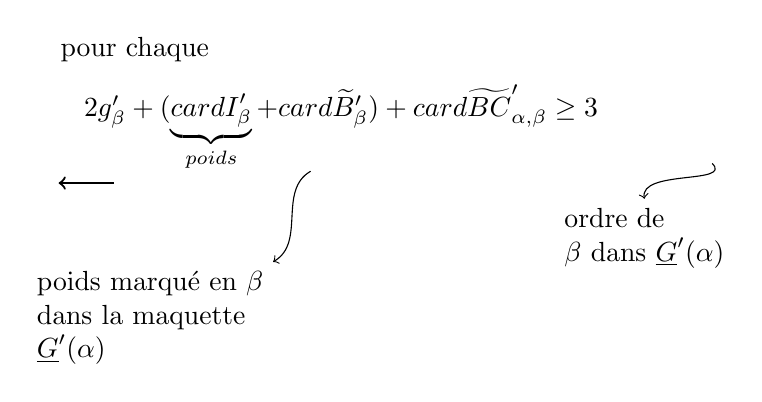
\begin{tikzpicture}[x=1cm,y=1cm]
\node[anchor=west] (eq) at (0,0) {$2g'_\beta+(\underbrace{\operatorname{card}I'_\beta}_{\deleted{\unsure{poids}}}\inserted{+\operatorname{card}\widetilde B'_\beta)}+\operatorname{card}\widetilde{\deleted{B}\inserted{C}}'_{\deleted{\unsure{\alpha}},\beta}\geq3$};
\node[anchor=north west,align=left] (mark) at (-0.6,-1.7) {poids marqué en $\beta$\\dans la maquette\\$\underline G'(\alpha)$};
\node[anchor=north west,align=left] (ord) at (6.1,-0.9) {ordre de\\$\beta$ dans $\underline G'(\alpha)$};
\draw[->,thick] (0.5,-0.7)--(-0.2,-0.7);
\draw[->] (3.0,-0.55) to[out=210,in=30] (mark.north east);
\draw[->] (8.1,-0.45) to[out=-45,in=100] (ord.north);
\node[anchor=west] at (-0.3,1.0) {\deleted{\unsure{pour chaque}}};
\end{tikzpicture}}

\margin{\unsure{car la condition est aut. assur.} \deleted{\unsure{a priori} $\unsure{2g'_\beta}$ \unsure{est}} \deleted{\unsure{puisqu'il est}} \unsure{équiv à} : \figure{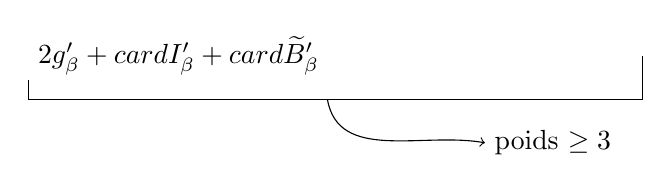
\begin{tikzpicture}[x=1cm,y=1cm]
\node[anchor=west] at (0,0) {$2g'_\beta+\operatorname{card}I'_\beta+\operatorname{card}\widetilde B'_\beta$};
\draw (0,-0.3)--(0,-0.55)--(7.8,-0.55)--(7.8,0);
\draw[->] (3.8,-0.55) to[out=-80,in=170] (5.8,-1.1);
\node[anchor=west] at (5.8,-1.1) {poids $\geq3$};
\end{tikzpicture}}}

\deleted{\unsure{qui a priori} \unsure{$+\operatorname{car}$} $\left[2g'_\beta+\operatorname{card}I'_\beta\geq3\right]$ $2g'_\beta+\operatorname{card}I'_\beta+\operatorname{card}\widetilde A'_\beta\geq3)$ qui a priori est une condition plus faible (puisque $\underline G'$ est un MD-graphe)\ldots}

d) le genre du MD-graphe $\underline G'(\alpha)$ est égal à $g_\alpha$, i.e. on a
\[
\sum_{\beta\in S'_\alpha}\unsure{g'_\beta|\gamma'_\beta}+h_1(G'(\alpha))=g_\alpha.
\]
\mspage{39}
\scanpage{41}
\uline{NB} Pour qu'un morphisme généralisé de graphes $G'\deleted{\unsure{\text{et}}}\longrightarrow G$ corresponde à un morphisme de générisation (pour $I'\simeq I$ convenable), il f. et s. qu'il satisfasse aux conditions suivantes
\[
(48)\quad\left\{\begin{aligned}
&\text{1°) }S'\unsure{\to|{-}}S\text{ surjectif},\quad\widetilde B'\longrightarrow\widetilde A\text{ bijectif, les}\\
&\qquad\inserted{\text{``graphes}}\text{ fibres'' }G'(\alpha)\quad(\alpha\in S)\text{ connexes. (Ces}\\
&\qquad\text{conditions ne dépendent pas des MD-}\\
&\qquad\text{structures sur }G',G\text{)}\\[1em]
&\text{2°) }\forall\alpha\in S,\text{ on a}\\
&\qquad\underbrace{\operatorname{card}I_\alpha}_{\nu_\alpha}=\sum_{\beta\in S'_\alpha}\underbrace{\operatorname{card}I'_\beta}_{\nu'_\beta}\\
&\qquad\text{(cette condition ne dépend que des}\\
&\qquad\text{``poids marqués'' sur }\unsure{\widehat S|S},S',\text{ et bien sûr}\\
&\qquad\text{de }S'\unsure{\to|{-}}S\text{)}\\[1em]
&\unsure{\text{3°)}}\quad\forall\alpha\in S,\text{ on a}\\
&\qquad g_\alpha=\Big(\sum_{\beta\in S'_\alpha}g'_\beta\Big)+h_1(G'(\alpha))\\[1em]
&\deleted{\unsure{\text{4°)}}\quad\forall\unsure{\beta|\alpha'}\in S',\text{ on a (non seulement}}\\
&\deleted{\quad2g'_{\alpha'}+\operatorname{card}I'_{\alpha'}+\operatorname{card}\widetilde A'_{\beta'}\geq3,\text{ mais même)}}\\
&\deleted{\qquad\unsure{2|7}g'_{\alpha}+\operatorname{card}I'_{\alpha'}+\operatorname{card}\unsure{\widetilde C'|\widetilde B'}_{\alpha'}\geq3}
\end{aligned}\right.
\]
\mspage{40}
\scanpage{42}
\mspage{20}
Reprenons un morphisme généralisé de graphes ordinaires $f:G'\to G^{\deleted{\unsure{'}}}$. On dit que $f$ est un \uline{morphisme de générisation} s'il satisfait la condition 1°) de (48). Notons que $G$ et $f$ sont définis alors à iso près par $G'$ et l'ens $\widetilde B'\subset\widetilde A'$ (stable par $\sigma_{\widetilde A'}$), ou ce qui revient au $\unsure{=|\overline m}$, par $G'$ et la \deleted{\unsure{ens}} partie $B'$ de $A'=\widetilde A'/\sigma_{\widetilde A'}$ ($B'$ est donc un ens. d'arêtes de $G'$). En effet, soit $G'_\bullet$ le sous-graphe de $G'$ défini par $S'$ et $A'\setminus B'\subset A'$ (ou $\widetilde A'\setminus\widetilde B'\subset\widetilde A'$) (i.e. \inserted{par $S'$ et} l'ens des \deleted{arêtes} arcs de $G'$ qui sont au dessus des identités de $\Pi_1(G)$). Alors il résulte de la condition $S'\unsure{\to|{-}}S$ surjectif et les $G'(\alpha)$ connexes ($\Longleftrightarrow$ les $G'(\alpha)$ 0-connexes) que \deleted{les fibres} l'homomorphisme canonique
\[
\pi_0(G'_\bullet)\longrightarrow S
\]
est bijectif, d'où
\[
(49)\qquad S\simeq\pi_0(G'_\bullet),
\]
d'ailleurs on a
\[
(50)\qquad\widetilde A\simeq\widetilde B'\qquad\unsure{\text{compatible}}\text{ avec }\sigma_{\widetilde B'}\text{ et }\sigma_{\widetilde A}
\]
\mspage{41}
\scanpage{43}
enfin $\widetilde A\xrightarrow{\unsure{o_G|\sigma_G}}S$ est donné par passage au quotient à partir de $o_G|\widetilde B':\widetilde B'\to S'$, par commutativité dans

(51)\quad\diagram{\begin{tikzcd}
\widetilde B'\arrow[r,"o_{G'}|\widetilde B'"]\arrow[d,"\unsure{\sim|\wr}"']&S'=\text{sommets de }G'_\bullet\arrow[d]\\
\widetilde A\arrow[r]&S\simeq\pi_0(G'_\bullet)
\end{tikzcd}}

Ainsi $G$ est reconstruit à partir de $G'$, et $f$ de $\unsure{\overline m|=}$ bien sûr. On voit que $G$ apparaît comme un quotient de $G'$, et en fait c'est plus une somme amalgamée dans la catégorie des graphes et des morphismes généralisés de graphes :

(52)\quad\diagram{\begin{tikzcd}[column sep=large,row sep=large]
G'_\bullet\arrow[r,hook,"\text{incl. can}"]\arrow[d,"\text{proj. can}"']\arrow[dr,phantom,"\text{cocart}"]&G'\arrow[d]\\
\begin{gathered}S=\pi_0(\unsure{G'_\bullet|S'_\bullet})\\
\text{Graphe }\deleted{\unsure{\text{ponctuel}}}\inserted{\text{discret}}\\
\text{défini par }S\overset{\mathrm{dfn}}{=}\pi_0(G'_\bullet)
\end{gathered}\arrow[r]&G
\end{tikzcd}}

i.e. $G'\longrightarrow G$ est universel parmi les morphismes généralisés de \inserted{$G$ dans un} graphe $G'$, qui transforment les arcs de $\widetilde A'\setminus\widetilde B'$ en des identités. Posons donc
\mspage{42}
\scanpage{44}
\mspage{21}
\[
(53)\qquad\widetilde C'=\widetilde A'\setminus\widetilde B',\qquad C'=A'\setminus B'=\widetilde C'/\sigma_{\widetilde A'},
\]
on écrira
\[
(54)\qquad G=G'/\widetilde C'\quad\text{ou}\quad G=G'/C'
\]
et on dira que $G$ \uline{est déduit de} $G'$ en contractant les arêtes $a'\in C'$ (ou encore, les arcs $\vec a'\in\widetilde C'$) en des pts. Interprétant les morphismes généralisés de graphes, en termes des réalisations \deleted{géométriques}\inserted{topologiques} de ceux-ci, à l'aide d'applications continues qui contractent juste certaines arêtes en des pts, on voit que cette terminologie correspond bien à une intuition topologique correcte. D'ailleurs la somme amalgamée (52) existe quel que soit le sous-graphe $G'_\bullet$ de $G'$ ayant $\unsure{=^{\mathrm s}|\overline m^{\mathrm s}}$ sommets que $G'$, i.e. quel que soit l'ens d'\deleted{flèches}\inserted{arêtes} $C'\subset A'$- de $G'_{\deleted{\unsure{\psi|\alpha}}\bullet}$. [Il s'ensuit que tout morphisme généralisé de graphes $G'\longrightarrow G$ se factorise de façon unique en un
\mspage{43}
\scanpage{45}
composé
\[
(55)\qquad G'\longrightarrow G_0\unsure{\longrightarrow|{-}}G,
\]
où $G'\unsure{\to|{-}}G_0$ est un morphisme de passage au quotient (par l'ens des arêtes de $G'$ contractées par $f$, justement) et où $G_0\longrightarrow G$ est un morphisme \inserted{ordinaire} de graphes.

Supposons maintenant que $G'$ \inserted{soit fixé, et} \deleted{soit} provienne \inserted{$\unsure{\overline m|=}$} d'un MD-graphe $\underline G'$, grâce aux données supplémentaires
\[
\deleted{\unsure{(55)|(56)}}\qquad I'\longrightarrow S',\xrightarrow{\unsure{g'|\underline{g'}}}\mathbb N,
\]
où $I'$ est un ens. fini. Alors $G$ provient canoniquement d'un MD-graphe $\underline G$, en posant $I=I_{\underline G}=I'$, et en définissant $\unsure{I|I'}\unsure{\to|{-}}S$ comme le composé
\[
\underset{\substack{\Vert\,\mathrm{déf}\\I}}{I'}\longrightarrow S'\unsure{\longrightarrow|{-}}S,
\]
et en définissant, pour $\forall\alpha\in S$
\[
(56)\qquad g_\alpha=\Big(\sum_{\alpha'\in\underset{\substack{\Vert\\\text{Sommets}\\\text{de }G'(\alpha)}}{S'_\alpha}}g'_{\alpha'}\Big)+h^1(G'(\alpha)).
\]
\mspage{44}
\scanpage{46}
\mspage{22}
Il faut cependant vérifier encore la condition MD sur la maquette $\underline G$ obtenue. Que $\underline G$ soit connexe résulte aussitôt de la connexité de $\underline G'$. Pour $\forall\alpha\in S$, il faut vérifier que
\[
2g_\alpha+\underbrace{\operatorname{card}I_\alpha+\operatorname{card}\widetilde A_\alpha}_{\widehat\nu_\alpha}\geq3
\]
\deleted{\unsure{or je dis qu'on aura mieux|ou je dis qu'on aura même}}

\deleted{ou}\inserted{i.e.} que $(g_\alpha,\widehat\nu_\alpha)$ est anabélien. Or
\[
\deleted{\operatorname{card}2g_\alpha+\operatorname{card}I_\alpha\geq3}
\]
\deleted{je dis}\inserted{on sait} que $(g_\alpha,\widehat\nu_\alpha)$ est le type numérique de la maquette $\underline{\unsure{G|G'}}(\alpha)$, dont le graphe sous-jacent est la composante connexe de $G'_\bullet$ correspondant à $\alpha$, et l'ens. des ``pts marqués'' est $I'_\alpha\amalg\deleted{\unsure{\widetilde A}}\inserted{\widetilde B}'_\alpha$, \deleted{\unsure{et|à}} où $I'_\alpha=I'|S'_\alpha\simeq I_\alpha$, et $\widetilde B'_\alpha=\deleted{\unsure{\widetilde B|\widetilde A}}\inserted{\unsure{\widetilde A|\widetilde B}}'_\alpha\cap\widetilde B'$ est l'ens des flèches $\in\widetilde B'$ d'origine dans $S'_\alpha$, l'hom de projection
\[
\unsure{I_{(\alpha)}|I^{(\alpha)}}^{\deleted{\unsure{\ast|\alpha}}}\overset{\mathrm{def.}}{=}I'_\alpha\amalg\widetilde B'_\alpha\longrightarrow S'_\alpha
\]
étant induit par $I'\to S'$ et l'application origine. Donc, en vertu de la prop. \unsure{de ce|du} n° 3, on aura $(g_\alpha,\widehat\nu_\alpha)$ anabélien pourvu qu'on sache que $\underline G(\alpha)$ est un MD-graphe. Mais cette condition signifie que l'on a, pour $\forall\beta\in S'_{\deleted{\unsure{\beta|\alpha'}}\inserted{\alpha}}$
\mspage{45}
\scanpage{47}
\[
2g'_\beta+\underbrace{\bigl(\operatorname{card}I'_\beta\deleted{\unsure{(\alpha)}}+\operatorname{card}\widetilde B'_{\unsure{\beta|\alpha}}\bigr)}_{\substack{\text{poids marqué}\\\text{de }\beta\text{ dans }\underline G(\alpha)}}+\underbrace{\operatorname{card}\widetilde C'_\beta}_{\substack{\text{ordre de}\\\beta\text{ dans }\underline G(\alpha)}}\geq3
\]
or cette expression s'écrit aussi, puisque
\[
\widetilde A'=\widetilde B'\amalg\widetilde C'
\]
\[
2g'_\beta+\underbrace{\operatorname{card}I'_\beta}_{\substack{\text{poids marqué}\\\text{de }\beta\text{ dans }\underline G'\deleted{\unsure{\alpha|\xi}}}}+\underbrace{\operatorname{card}\widetilde A_\beta}_{\substack{\text{ordre de }\beta\\\text{dans }\underline G'}}\geq3,
\]
et cette condition n'est autre que la condition \inserted{de rigidité} MD sur $\underline G'$.

Résumons les résultats sur les maquettes.

\uline{Proposition}\quad Soit
\[
\underline G'=\left(\underset{\substack{\Vert\\(S',\deleted{\unsure{\widetilde B}}\inserted{\widetilde A}',\sigma_{\widetilde A'},o_{\widetilde A'})}}{G'},\ I'\longrightarrow S'\xrightarrow{\unsure{g'|\underline{g'}}}\mathbb N\right)
\]
une maquette, et soit $C'\subset A'=\widetilde A'/\sigma_{\widetilde A'}$ un ens d'arêtes de $G'$. Alors on peut de façon unique \deleted{trouver} (à isom unique près) trouver un morphisme de générisation de maquettes
\[
\underline G'\longrightarrow\underline G
\]
\mspage{46}
